\documentclass[runningheads]{llncs}

\usepackage[T1]{fontenc}

\usepackage[utf8]{inputenc}

\usepackage{newtxtext}

\usepackage[varvw]{newtxmath}

\usepackage{graphicx}

\usepackage{amsmath}

\usepackage{url}

\usepackage{array}

\begin{document}

\title{Interpretable Cognitive Load Classification Using Fuzzy Time-Series, ANFIS, and Bayesian Network Fusion}

\titlerunning{Interpretable Cognitive Load Classification}

\author{Quoc-Huy Nguyen\inst{1}\thanks{Corresponding author: dntai@sgu.edu.vn} \and Nhu-Tai Do\inst{1} \and Le Thi My Huong\inst{1} \and Quan Do Minh\inst{1}}

\authorrunning{Q.-H. Nguyen et al.}

\institute{Faculty of Information Technology, Sai Gon University, Viet Nam}

\maketitle

\begin{abstract}

Cognitive load monitoring is important in human-computer interaction, education, and healthcare, but wearable physiological signals are often noisy, subject-dependent, and overlapping across cognitive states. This study proposes an interpretable FTS-ANFIS-BN framework for cognitive load classification using heart rate, respiration rate, galvanic skin response, and skin temperature from the CogLoad dataset. The framework captures temporal dynamics through soft fuzzy time-series transitions, learns signal-specific nonlinear evidence using ANFIS models, and combines multi-signal information through soft-evidence Bayesian fusion. Experimental results on an independent subject-level test set show that the proposed model achieves 75.13\% accuracy and 77.34\% ROC-AUC, outperforming all controlled classical machine-learning baselines evaluated under the same subject-independent protocol. The framework also enables interpretation through fuzzy-transition patterns, ANFIS consequent coefficients, and Bayesian evidence likelihoods. These results indicate that integrating fuzzy temporal representation, neuro-fuzzy learning, and probabilistic evidence fusion can provide effective and interpretable wearable-based cognitive load classification.

\keywords{Cognitive load, Fuzzy time series, ANFIS, Bayesian network, Wearable physiological signals, Explainable classification}

\end{abstract}


\section{Introduction}

Cognitive load refers to the mental effort required to process information within the limited capacity of working memory \cite{ref1}. Excessive cognitive load can adversely affect attention, learning, decision-making, and task performance, making its assessment important in education, healthcare, human-computer interaction, and occupational safety \cite{ref1,ref2,ref3,ref4}. In practical monitoring systems, cognitive load is often represented using simplified levels or binary states such as REST and TASK, thereby formulating the problem as a classification task \cite{ref2}.

Recent advances in wearable sensing enable continuous and non-intrusive acquisition of physiological signals related to cognitive activity, including heart rate (HR), respiration rate (RR), galvanic skin response (GSR), and skin temperature (Temp) \cite{ref2}, \cite{ref3}. The CogLoad benchmark uses these signals for REST-versus-TASK cognitive load classification \cite{ref3}. However, reliable classification remains challenging because physiological responses are noisy, subject-dependent, and often overlap across cognitive states.

Existing approaches commonly rely on fixed-window statistical summaries, which may not explicitly represent temporal changes occurring within a physiological segment. More complex machine-learning models can capture nonlinear relationships but may provide limited insight into how temporal patterns and individual physiological channels contribute to the final prediction. Therefore, an effective cognitive load classification framework should capture temporal transitions, model nonlinear and uncertain physiological responses, and preserve interpretable signal-level evidence.

Fig. 1 illustrates the motivation of this study. Cognitive activities such as learning, problem solving, and task execution induce physiological responses that can be observed through wearable sensors. Because the resulting patterns may overlap between REST and TASK conditions, an interpretable framework is required to represent temporal signal evolution, learn signal-specific evidence, and combine information from multiple physiological sources in a transparent manner.

\begin{figure}[t]

\centering

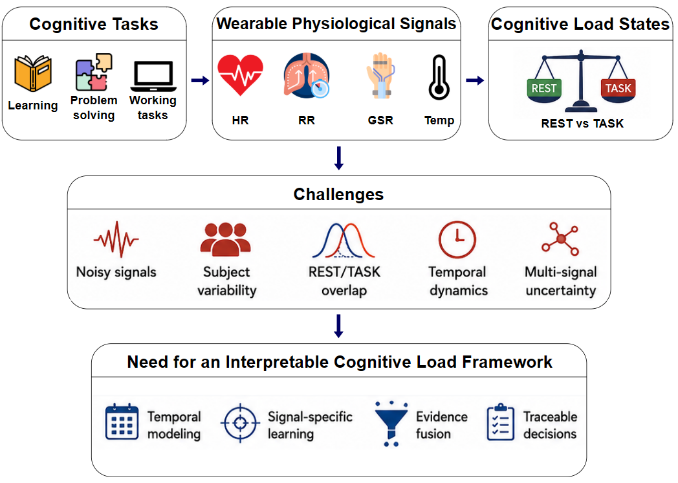
\includegraphics[width=\linewidth]{figures/figure1.png}

\caption{Motivation for wearable-based cognitive load classification.}\label{fig:rId11}

\end{figure}

Motivated by these challenges, this study proposes an interpretable FTS-ANFIS-BN framework for cognitive load classification using wearable physiological signals. The framework integrates Fuzzy Time Series (FTS), Adaptive Neuro-Fuzzy Inference System (ANFIS), and Bayesian Network (BN) modelling. FTS is used to represent temporal state transitions through soft fuzzy relations \cite{ref5}, \cite{ref6}. Signal-specific ANFIS models then learn nonlinear relationships between fuzzy-transition patterns and cognitive states \cite{ref7}. Finally, the resulting signal-level outputs are combined through soft-evidence Bayesian fusion to estimate the posterior probabilities of REST and TASK \cite{ref8}.

Rather than treating FTS, ANFIS, and Bayesian modelling as independent components, the proposed framework connects them through an interpretable evidence representation. Temporal information is first encoded as soft fuzzy-transition matrices, transformed into signal-specific cognitive-load evidence by ANFIS, and subsequently fused probabilistically using quantile-based soft evidence. This design provides interpretable information at the temporal-transition, signal, and probabilistic-evidence levels.

The main contributions of this study are summarized as follows:

1. A soft fuzzy-transition representation is proposed by combining consecutive fuzzy membership vectors to construct a row-normalized 3 $\times$ 3 transition matrix for each physiological signal. The resulting representation provides nine interpretable temporal features per signal and 36 features for each four-signal window.

2. Four signal-specific first-order TSK ANFIS models are employed to transform the fuzzy-transition features of HR, RR, GSR, and Temp into signal-level cognitive-load evidence while preserving access to the learned premise and consequent parameters for interpretation.

3. A soft-evidence Bayesian fusion mechanism is introduced to combine the four signal-level outputs using five quantile-based evidence states, additively smoothed conditional probability tables, and posterior inference for REST and TASK classification.

\section{Related works}

Cognitive load assessment has been widely studied in education, healthcare, human-computer interaction, and wearable computing. Traditional methods often rely on subjective self-report instruments such as the NASA Task Load Index \cite{ref4}. Although useful for perceived workload assessment, these methods are typically administered after task completion and may be influenced by recall bias and individual perception. This has motivated objective and continuous cognitive load monitoring using physiological signals.

Wearable sensing enables the collection of physiological signals associated with cognitive activity, including HR, RR, GSR, and Temp \cite{ref2}. The CogLoad dataset and the UbiComp 2020 Cognitive Load Monitoring Challenge established a benchmark for REST/TASK classification \cite{ref3}. The best-reported challenge method achieved 69.4\% accuracy using an ensemble of gradient-boosting decision trees \cite{ref3}. However, most challenge approaches relied on handcrafted statistical features from fixed-length windows, which may not explicitly capture temporal transitions within physiological segments. Therefore, this result is used here as a contextual literature reference rather than as a directly controlled baseline.

Recent studies have also highlighted inter-subject variability, measurement conditions, synchronization issues, environmental variability, ground-truth reliability, feature selection, and validation strategy as important challenges in wearable cognitive-workload monitoring \cite{ref9,ref10,ref11}. These findings motivate subject-independent evaluation and careful control of model-selection procedures.

Machine-learning and deep-learning methods can model complex physiological patterns, but noisy and subject-dependent signals remain challenging, and complex models may provide limited transparency \cite{ref12}. Fuzzy methods are useful for representing gradual and overlapping states. ANFIS combines data-driven learning with interpretable fuzzy rules \cite{ref7} and has been applied to cognitive-signal modelling \cite{ref13}, while fuzzy features have also been used for overlapping EEG patterns \cite{ref14}. However, these studies mainly concern EEG or multimodal brain signals rather than wrist-derived HR, RR, GSR, and Temp under the CogLoad protocol.

FTS represents uncertain temporal processes through fuzzy states and relations \cite{ref5}, \cite{ref6}. Although recent FTS research includes alternative partitions, higher-order relations, probabilistic formulations, and hybrid learning \cite{ref15}, most applications focus on forecasting. In this study, fuzzy transitions are instead used to describe within-window physiological-state evolution.

Bayesian networks provide a probabilistic framework for reasoning under uncertainty and are suitable for combining complementary physiological evidence \cite{ref8}. Previous fuzzy-Bayesian approaches have been applied in other uncertainty-analysis domains \cite{ref16}, but with different variables, objectives, and inference settings.

Overall, existing approaches still leave three related limitations: static features may overlook temporal transitions, complex classifiers may provide limited evidence-level interpretability, and multi-signal evidence may not be fused transparently. The proposed FTS-ANFIS-BN framework addresses these gaps through fuzzy temporal encoding, signal-specific neuro-fuzzy inference, and soft-evidence Bayesian fusion under subject-independent evaluation.

\section{Materials and methods}

\subsection{Dataset and experimental protocol}

The experiments were conducted using the publicly available CogLoad dataset \cite{ref2}, collected from 23 participants wearing a wrist-worn sensing device on the non-dominant arm. Four physiological signals were used: Temp, HR, GSR, and RR. The dataset contains 825 labelled samples, with REST assigned to class 0 and TASK to class 1. Table 1 summarizes the dataset characteristics and evaluation split.

\begin{table}[t]
\centering
\caption{Summary of the CogLoad data.}\label{tab:1}
\small
\begin{tabular}{lc}
\hline
Item & Description \\
\hline
Participants & 23 participants \\
Total samples & 825 samples \\
Physiological signals & Temp, HR, GSR, and RR \\
Development set & 632 samples from 18 participants \\
Independent test set & 193 samples from 5 participants \\
Segment length & Final 30 seconds of each REST or TASK episode \\
Labels & REST = 0 and TASK = 1 \\
\hline
\end{tabular}
\end{table}

\begin{figure}[t]

\centering

Fig. 2 shows the three-stage FTS-ANFIS-BN framework for temporal representation, signal-specific nonlinear learning, and interpretable probabilistic fusion.

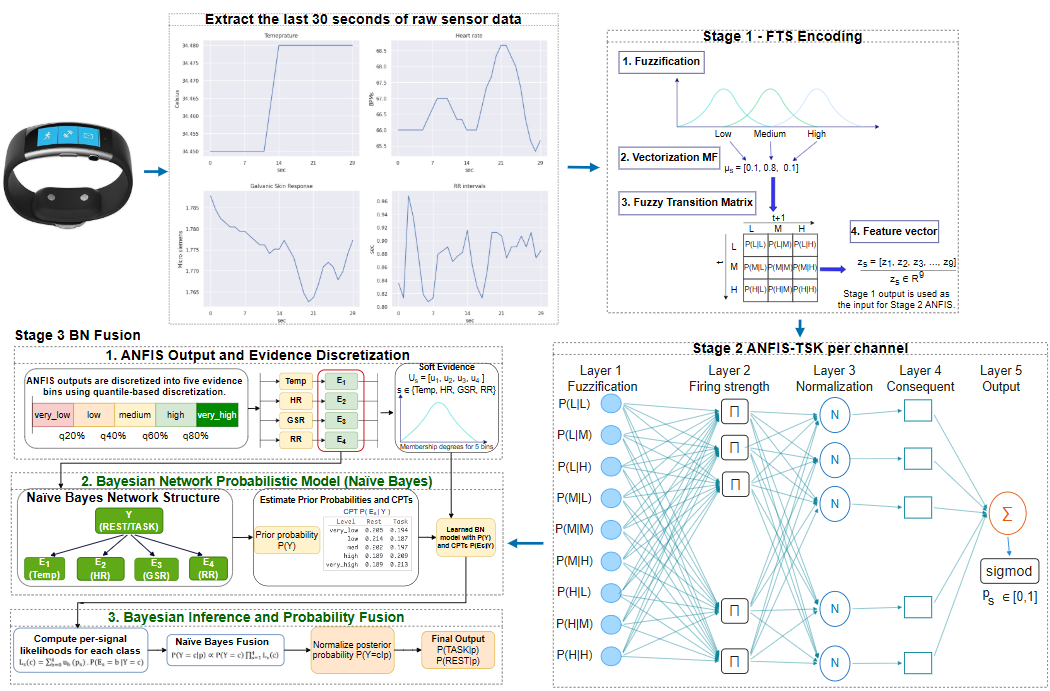
\includegraphics[width=\linewidth]{figures/figure2.png}

\caption{Overall pipeline of the proposed FTS--ANFIS--BN method.}\label{fig:rId13}

\end{figure}

The experimental protocol included working-memory and elementary cognitive tasks designed to induce different cognitive demands, followed by NASA-TLX assessment \cite{ref4}. Each sample represents the final 30 seconds of a REST or TASK episode. Following the predefined CogLoad partition \cite{ref3}, also adopted in a later wristband-based study \cite{ref17}, 632 samples from 18 participants were used for model development and 193 samples from five unseen participants were reserved for independent testing, with no participant overlap. The development set was used for subject-wise cross-validation, model selection, and threshold optimization, whereas the test set was used exclusively for final evaluation. Further details are provided in Section 3.6.

\subsection{Proposed framework}

First, each 30-second Temp, HR, GSR, and RR segment is fuzzified into three states and represented by a normalized fuzzy-transition matrix. Second, a signal-specific first-order TSK ANFIS model maps the transition features of each physiological signal to a TASK evidence score. Third, the four signal-level scores are represented as soft evidence and combined using a Bayesian network with a Naive Bayes topology. The final REST/TASK label is obtained from the posterior probability using a decision threshold selected exclusively from training-subject out-of-fold predictions.

Interpretability is provided at multiple levels through FTS transition matrices, ANFIS rule activations and consequent parameters, and Bayesian priors, conditional probability tables (CPTs), evidence likelihoods, and posterior probabilities.

\subsection{Fuzzy time series encoding}

For each signal, the raw segment is fuzzified into K = 3 states: low, medium, and high. All membership parameters are estimated from fold-training data. The universe is defined from the observed training range and expanded by 5\% at both boundaries. Three centers are evenly spaced over this interval, and the Gaussian width is set to 0.4 times the distance between adjacent centers \cite{ref5}, \cite{ref15}.

Gaussian memberships are computed by Eq. (1) and normalized by Eq. (2), producing a soft partition whose memberships sum to one at each time point \cite{ref7}, \cite{ref18}.

\begin{equation}\mu_{s,k}^{\mathrm{raw}}(x)=\exp\!\left(-\frac{(x-c_{s,k})^2}{2\sigma_s^2}\right)\tag{1}\end{equation}

\begin{equation}\mu_{s,k}(x)=\frac{\mu_{s,k}^{\mathrm{raw}}(x)}{\sum_{k\prime=1}^{K}\mu_{s,k\prime}^{\mathrm{raw}}(x)}\tag{2}\end{equation}

At time t, signal xs(t) is represented by the membership vector

The vector retains partial memberships instead of assigning only the maximum state.

A K x K transition matrix is then constructed from consecutive membership vectors. Each Tij\textasciicircum{}(s) accumulates the product t-norm for transitions from state i at t to state j at t+1. This adapts Cartesian-product fuzzy relations \cite{ref6} to consecutive observations, as shown in Eqs. (3) and (4).

\begin{equation}R^{(s)}\approx\bigcup_{k=1}^{C}\left(A^{(k)}\times B^{(k)}\right)\tag{3}\end{equation}

\begin{equation*}\mathbf{T}^{(s)}=\sum_{t=1}^{L-1}\boldsymbol{\mu}_s(t)^{\mathsf T}\boldsymbol{\mu}_s(t+1)\end{equation*}

\begin{equation}T_{ij}^{(s)}=\sum_{t=1}^{L-1}\mu_{s,i}(x_s(t))\,\mu_{s,j}(x_s(t+1))\tag{4}\end{equation}



\begin{equation}\mathbf{T}^{(s)}=\begin{bmatrix}T_{L,L}^{(s)}&T_{L,M}^{(s)}&T_{L,H}^{(s)}\\T_{M,L}^{(s)}&T_{M,M}^{(s)}&T_{M,H}^{(s)}\\T_{H,L}^{(s)}&T_{H,M}^{(s)}&T_{H,H}^{(s)}\end{bmatrix}\tag{5}\end{equation}

Each row is normalized by Eq. (6), yielding a probability-like next-state distribution conditioned on the current fuzzy state. The matrix is then flattened into nine transition features.

\begin{equation}\widetilde{T}_{ij}^{(s)}=\frac{T_{ij}^{(s)}}{\sum_{j\prime=1}^{K}T_{ij\prime}^{(s)}}\tag{6}\end{equation}

Thus, four signals produce 36 smooth, interpretable transition features while retaining all membership degrees.

\subsection{Signal-specific ANFIS classifiers}

The second stage trains one ANFIS model per physiological signal \cite{ref7}. Each model receives nine FTS features, allowing signal-level evidence to be inspected before Bayesian fusion.

\begin{equation*}\mathbf{z}^{(s)}=[z_1^{(s)},z_2^{(s)},\ldots,z_d^{(s)}]^{\mathsf T},\quad d=9\end{equation*}

Each signal-specific model uses R first-order TSK rules with Gaussian premises \cite{ref7}, \cite{ref19}:

\begin{equation}R_r^{(s)}:\;\text{IF }z_1^{(s)}\text{ is }A_{r,1}^{(s)}\text{ AND }\cdots\text{ AND }z_d^{(s)}\text{ is }A_{r,d}^{(s)}\text{ THEN }f_r^{(s)}(\mathbf z)=\sum_{j=1}^{d}a_{r,j}^{(s)}z_j^{(s)}+b_r^{(s)}\tag{7}\end{equation}

Here, s, r, and j index the signal, rule, and FTS feature; the consequent coefficients and bias are learned from data.

Gaussian premise membership is calculated as:

\begin{equation}\mu_{r,j}^{(s)}(z_j^{(s)})=\exp\!\left[-\frac{(z_j^{(s)}-c_{r,j}^{(s)})^2}{2(\sigma_{r,j}^{(s)})^2}\right]\tag{8}\end{equation}

The product t-norm gives each rule firing strength:

\begin{equation}w_r^{(s)}=\prod_{j=1}^{d}\mu_{r,j}^{(s)}(z_j^{(s)})\tag{9}\end{equation}

Firing strengths are normalized across the R rules:

\begin{equation}\bar{w}_r^{(s)}=\frac{w_r^{(s)}}{\sum_{r\prime=1}^{R}w_{r\prime}^{(s)}}\tag{10}\end{equation}

The raw ANFIS output is the normalized weighted sum of the linear consequents:

\begin{equation}y_s=\sum_{r=1}^{R}\bar{w}_r^{(s)}f_r^{(s)}(\mathbf z)\tag{11}\end{equation}

A sigmoid map the raw output to [0,1]:

\begin{equation}p_s=\frac{1}{1+\exp(-y_s)},\quad 0\le p_s\le1\tag{12}\end{equation}

The resulting ps is a signal-level TASK evidence score; the four models output pTemp, pHR, pGSR, and pRR. Within each fold, K-means initializes rule centers and within-cluster standard deviations initialize Gaussian widths.

Hybrid learning estimates consequent parameters by ridge-regularized least squares and updates premise centers and widths by gradient descent, using fold-training data only. Rules are learned rather than manually specified. Absolute consequent-coefficient magnitudes support feature-use inspection but are not interpreted as causal contributions to the final BN posterior.

\subsection{Bayesian network fusion}

The BN uses a Naive Bayes structure, with cognitive load as the parent of the Temp, HR, GSR, and RR evidence nodes.

\subsubsection{Quantile-based discretization}

Each ANFIS score in [0,1] is partitioned into B = 5 quantile bins using fold-training scores only \cite{ref20}. The internal boundaries are the 20th, 40th, 60th, and 80th percentiles (Eq. (13)).

\begin{equation}\mathrm{boundaries}_s=[q_{s,20},q_{s,40},q_{s,60},q_{s,80}]\tag{13}\end{equation}

The five intervals are (-$\infty$, q20), [q20, q40), [q40, q60), [q60, q80), and [q80, +$\infty$), labeled very low to very high. These labels describe ANFIS-evidence levels rather than physiological states. Approximately balanced bin frequencies support stable and interpretable CPT estimation.

\subsubsection{Prior and conditional probability estimation}

Class priors and evidence-node CPTs are estimated from fold-training data with additive smoothing $\alpha$ = 0.5 to avoid zero probabilities \cite{ref21}.

Let N\_c denote the class count and N(s,b,c) the count for signal s, bin b, and class c. Eqs. (14) and (15) give the smoothed prior and CPT.

\begin{equation}P(CL=c)=\frac{N_c+\alpha}{N+2\alpha}\tag{14}\end{equation}

\begin{equation}P(E_s=b\mid CL=c)=\frac{N_{s,b,c}+\alpha}{N_c+B\alpha},\quad B=5\tag{15}\end{equation}

Under conditional independence, the joint distribution factorizes as Eq. (16), allowing each signal likelihood to be inspected separately.

\begin{equation}P(CL,E_1,E_2,E_3,E_4)=P(CL)\prod_{s\in\{\mathrm{Temp,HR,GSR,RR}\}}P(E_s\mid CL)\tag{16}\end{equation}

The four evidence variables correspond to Temp, HR, GSR, and RR.

During cross-validation, priors, boundaries, and CPTs were re-estimated within each training fold. After configuration selection, they were learned from all 632 development samples for hold-out evaluation. Reported probabilities were rounded to four decimals.

\subsubsection{Soft-evidence inference}

Although hard evidence states are used to estimate the CPTs, a new ANFIS score is not assigned exclusively to a single evidence bin during inference. Instead, it is represented as a soft distribution over all five evidence bins, following uncertain-evidence reasoning in Bayesian networks \cite{ref22}. For each signal, the lower and upper training-score limits are combined with the four quantile boundaries to form five bin intervals. The midpoint m(s,b) of each interval is then calculated. The Gaussian kernel value for evidence bin b is defined as:

\begin{equation*}k_{s,b}(p_s)=\exp\!\left[-\frac{1}{2}\left(\frac{p_s-m_{s,b}}{\sigma_s}\right)^2\right]\end{equation*}

The five kernel values are normalized to obtain the soft membership of score p\_s in evidence bin b:

\begin{equation}\mu_{s,b}(p_s)=\frac{k_{s,b}(p_s)}{\sum_{b\prime=1}^{5}k_{s,b\prime}(p_s)}\tag{17}\end{equation}

Therefore, the five soft memberships of each signal sum to one. For cognitive load class c, the likelihood contributed by signal s is obtained by weighting the learned CPT values with the corresponding soft memberships:

\begin{equation}L_s(c\mid p_s)=\sum_{b=1}^{5}\mu_{s,b}(p_s)P(E_s=b\mid CL=c)\tag{18}\end{equation}

This operation allows evidence near a quantile boundary to support neighboring bins instead of producing an abrupt hard assignment. The four signal-specific likelihoods are then combined with the class prior. For each class c, an unnormalized class score is computed as:

The normalized Bayesian posterior is then calculated as follows:

\begin{equation}P(CL=c\mid\mathbf p)=\frac{g_c}{g_{\mathrm{REST}}+g_{\mathrm{TASK}}}\tag{19}\end{equation}

The final output is P(CL = TASK | p). Its threshold is selected only from training-subject OOF predictions; the test set is not used for binning, priors, CPTs, soft-evidence parameters, or threshold selection.

\subsection{Experimental configurations}

All experiments followed the predefined subject-independent CogLoad split, with 632 samples from 18 participants used for model development and 193 samples from five unseen participants reserved for final testing. Five-fold GroupKFold cross-validation was performed at the participant level, and the same folds were used across all model configurations, ablation studies, and baseline methods. To prevent data leakage, all data-dependent operations were fitted exclusively on the training portion of each fold. Out-of-fold predictions were used for model comparison and decision-threshold selection, with the threshold chosen to maximize balanced accuracy over the range 0.05--0.95 in increments of 0.005. After model selection, the chosen pipeline was retrained on the full development set and evaluated once on the independent hold-out test set. Table 2 summarizes the evaluated configurations.

\begin{table}[t]
\centering
\caption{Experimental configurations}\label{tab:2}
\small
\begin{tabular}{lc}
\hline
Configuration & Values \\
\hline
FTS membership function & Triangular, Gaussian, trapezoidal, generalized bell \\
Number of ANFIS rules & 3, 6, 8, 12 \\
Component ablation & Full FTS-ANFIS-BN, FTS-ANFIS-Mean, and FTS Summary-BN \\
Machine-learning baselines & Statistical LR, RBF SVM, Random Forest, HistGradientBoosting, and Flattened-window LR \\
\hline
\end{tabular}
\end{table}

\begin{table}[t]
\centering
\caption{Parameter values used in the reference FTS-ANFIS-BN configuration}\label{tab:3}
\small
\begin{tabular}{lcc}
\hline
Section & Parameter & Value \\
\hline
FTS encoding & Number of fuzzy states & 3 \\
 & Universe expansion margin & 5\% \\
 & Gaussian width scale & 0.4 \\
 & Transition normalization & Row normalization \\
 & Number of transition features per signal & 9 \\
ANFIS training & K-means initializations & 10 \\
 & Initial premise-width scale & 1.3 \\
 & Number of training epochs & 50 \\
 & Learning rate & 0.003 \\
 & Ridge regularization coefficient & 0.01 \\
Bayesian network fusion & Network structure & Naive Bayes \\
 & Number of evidence bins & 5 \\
 & Discretization method & Quantile-based \\
 & Additive smoothing coefficient & 0.5 \\
 & Evidence-inference method & Soft evidence \\
\hline
\end{tabular}
\end{table}

FTS-ANFIS-Mean removes the Bayesian fusion stage and uses the arithmetic mean of the four signal-specific ANFIS scores as the final evidence score. In contrast, FTS Summary-BN removes the ANFIS stage and replaces it with predefined summaries derived from the FTS transition matrices, while retaining the Bayesian fusion stage.

The statistical machine-learning baselines used six features per signal mean, standard deviation, minimum, maximum, range, and linear trend resulting in 24 features in total. For the flattened-window logistic regression baseline, the four 30-point physiological sequences were concatenated into a 120-dimensional input vector.

ANFIS models were trained for 50 epochs without early stopping. For hyperparameter and ablation comparisons, only the investigated component was varied while the remaining settings were kept fixed. All methods used the same subject-independent split, participant-wise cross-validation folds, fold-local fitting procedure, out-of-fold threshold selection, and final hold-out evaluation. The reference parameter settings are summarized in Table 3.

\section{Results and Discussion}

\subsection{Hyperparameter selection}

Membership-function type and rule-base size were jointly selected from development-set OOF predictions. All 16 combinations of four membership functions and 3, 6, 8, or 12 rules used the complete pipeline with all other settings fixed. Each configuration used the OOF balanced-accuracy threshold search defined in Section 3.6.

\begin{table}[t]
\centering
\caption{Joint selection of FTS membership function and ANFIS rule-base size based on OOF balanced accuracy.}\label{tab:4}
\small
\begin{tabular}{lcccc}
\hline
Membership function & 3 rules & 6 rules & 8 rules & 12 rules \\
\hline
Triangular & 0.6032 & 0.6055 & 0.5858 & 0.5885 \\
Gaussian & 0.6047 & 0.6236 & 0.5795 & 0.5557 \\
Trapezoidal & 0.5978 & 0.6111 & 0.6080 & 0.5790 \\
Generalized bell & 0.5658 & 0.5763 & 0.5844 & 0.5558 \\
\hline
\end{tabular}
\end{table}

Table 4 shows that Gaussian membership with six rules achieved the highest OOF balanced accuracy (0.6236). Its threshold of 0.55 and all model choices were locked before full-development retraining and hold-out evaluation.

\subsection{Test set results}

The selected model was retrained on all 632 development samples and evaluated once, with the locked threshold 0.55, on 193 samples from five unseen participants.

\begin{table}[t]
\centering
\caption{Performance of the proposed FTS-ANFIS-BN model on the independent hold-out test set.}\label{tab:5}
\small
\begin{tabular}{lc}
\hline
Metric & Value \\
\hline
Accuracy & 0.7513 \\
Balanced Accuracy & 0.7519 \\
Precision & 0.7778 \\
Recall & 0.7143 \\
TASK F1-score & 0.7447 \\
Macro-F1 & 0.7511 \\
ROC-AUC & 0.7734 \\
\hline
\end{tabular}
\end{table}

As shown in Table 5, the proposed model achieved an accuracy of 0.7513 and a balanced accuracy of 0.7519. The similar accuracy, balanced accuracy, and Macro-F1 values indicate relatively balanced classification performance across the REST and TASK classes. For the TASK class, the model obtained a precision of 0.7778, a recall of 0.7143, and an F1-score of 0.7447. The ROC-AUC of 0.7734 further demonstrates the discriminative ability of the model outputs independently of the selected decision threshold.

\begin{figure}[t]

\centering

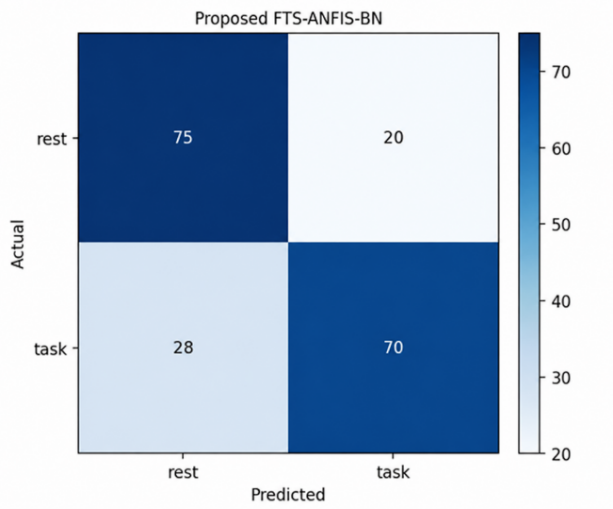
\includegraphics[width=\linewidth]{figures/figure3.png}

\caption{Confusion matrix of the proposed FTS--ANFIS--BN model on the independent hold-out test set.}\label{fig:rId15}

\end{figure}

The corresponding confusion matrix is presented in Fig. 3. As shown in Fig. 3, the model correctly classified 145 of the 193 test samples. Specifically, 75 of 95 REST samples and 70 of 98 TASK samples were correctly classified. The remaining errors consisted of 20 REST samples classified as TASK and 28 TASK samples classified as REST. To quantify uncertainty, 95\% confidence intervals for the main test metrics were estimated using 10,000 subject-clustered bootstrap replicates with random seed 4242. Participants, rather than individual samples, were resampled to preserve within-subject dependence. The corresponding 95\% confidence intervals were [0.7047, 0.8144] for accuracy, [0.7052, 0.8156] for balanced accuracy, [0.6854, 0.8141] for TASK F1-score, and [0.7368, 0.8062] for ROC-AUC.

\subsection{Baseline comparison and ablation analysis}

The proposed FTS-ANFIS-BN framework was compared with five conventional machine-learning baselines using the same subject-independent development and hold-out test partitions. Statistical Logistic Regression, RBF SVM, Random Forest, and HistGradientBoosting were trained using 24 statistical features, including the mean, standard deviation, minimum, maximum, range, and linear trend of each physiological signal. Flattened-window Logistic Regression directly used the four 30-point physiological sequences concatenated into a 120-dimensional input vector. Table 6 presents the results on the independent hold-out test set.

Among the controlled baselines evaluated under the same protocol, the proposed model achieved the highest values for all reported metrics. Random Forest was the strongest baseline, with an accuracy of 0.6891, a balanced accuracy of 0.6890, and a ROC-AUC of 0.7126. Compared with Random Forest, the proposed model improved these metrics by 0.0622, 0.0629, and 0.0608, respectively. The lower performance of flattened-window Logistic Regression further suggests that directly applying a simple linear classifier to raw temporal samples may be insufficient to capture the temporal structure relevant to cognitive-load classification.

\begin{table}[t]
\centering
\caption{Comparison with machine-learning baselines on the independent hold-out test set}\label{tab:6}
\small
\begin{tabular}{lcccc}
\hline
Model & Acc. & Bal. Acc. & TASK F1 & ROC-AUC \\
\hline
Proposed FTS-ANFIS-BN & 0.7513 & 0.7519 & 0.7447 & 0.7734 \\
Statistical Logistic Regression & 0.6373 & 0.6369 & 0.6500 & 0.7126 \\
RBF SVM & 0.6269 & 0.6252 & 0.6667 & 0.7126 \\
Random Forest & 0.6891 & 0.6890 & 0.6939 & 0.7126 \\
HistGradientBoosting & 0.6062 & 0.6061 & 0.6122 & 0.6455 \\
Flattened-window Logistic Regression & 0.5492 & 0.5442 & 0.6615 & 0.5454 \\
\hline
\end{tabular}
\end{table}

An ablation analysis was conducted to assess the contribution of the main components of the proposed framework. In FTS-ANFIS-Mean, Bayesian-network fusion was replaced by the arithmetic mean of the four ANFIS evidence scores. In FTS Summary-BN, the signal-specific ANFIS models were replaced by predefined summary scores derived from the FTS transition matrices, while Bayesian fusion was retained. The ablation results are presented in Table 7.

\begin{table}[t]
\centering
\caption{Ablation results on the independent hold-out test set.}\label{tab:7}
\small
\begin{tabular}{lcccc}
\hline
Configuration & Acc. & Bal. Acc. & TASK F1 & ROC-AUC \\
\hline
Proposed FTS-ANFIS-BN & 0.7513 & 0.7519 & 0.7447 & 0.7734 \\
FTS--ANFIS--Mean & 0.6891 & 0.6873 & 0.7248 & 0.7158 \\
FTS Summary--BN & 0.5389 & 0.5385 & 0.5528 & 0.5709 \\
\hline
\end{tabular}
\end{table}

Replacing BN fusion with averaging reduced balanced accuracy from 0.7519 to 0.6873 and ROC-AUC from 0.7734 to 0.7158. Replacing ANFIS with FTS summaries caused a larger decline to 0.5385 balanced accuracy and 0.5709 ROC-AUC, supporting the complementary roles of ANFIS inference and Bayesian fusion.

\subsection{Participant-wise test results}

To examine performance variation across unseen individuals, the final model was evaluated separately for each of the five participants in the independent hold-out test set. The same locked model and decision threshold of 0.55 were applied to all participants, without participant-specific retraining or threshold adjustment. The participant-wise results are presented in Table 8.

\begin{table}[t]
\centering
\caption{Participant-wise test performance of the proposed model.}\label{tab:8}
\small
\begin{tabular}{lccc}
\hline
Participant & N & Acc. & ROC-AUC \\
\hline
3caqi & 39 & 0.6923 & 0.7842 \\
6frz4 & 39 & 0.7179 & 0.7237 \\
bd47a & 38 & 0.7105 & 0.7452 \\
f1gjp & 39 & 0.8718 & 0.8026 \\
iz3x1 & 38 & 0.7632 & 0.8366 \\
\hline
\end{tabular}
\end{table}

Participant-wise accuracy ranged from 0.6923 to 0.8718, with mean 0.7511 $\pm$ 0.0647; mean ROC-AUC was 0.7785 $\pm$ 0.0403. These results show that classification performance varied across participants, although the same locked model and threshold were used in all cases. The participant-wise analysis was conducted only after final model selection and was not used for hyperparameter tuning or threshold optimization.

\subsection{Model interpretation}

\subsubsection{Interpretation of FTS transition patterns}

\begin{figure}[t]

\centering

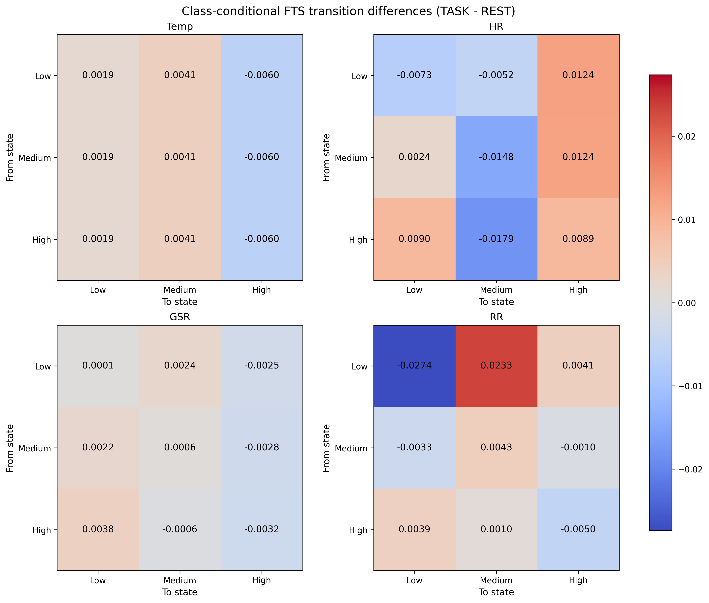
\includegraphics[width=\linewidth]{figures/figure4.png}

\caption{Class-conditional differences in mean fuzzy transition matrices for the four physiological signals.}\label{fig:rId16}

\end{figure}

As shown in Fig. 4, RR exhibited the largest class-conditional differences: Low-to-Low transitions were more prominent in REST (-0.0274), whereas Low-to-Medium transitions were more prominent in TASK (0.0233). HR also showed stronger transitions toward the High state in TASK, while Temp and GSR exhibited smaller differences. These findings confirm that the FTS stage captured signal-specific temporal patterns distinguishing REST from TASK.

\subsubsection{Interpretation of ANFIS consequent coefficients}

Fig. 5 presents the summed absolute magnitudes of the consequent coefficients associated with the nine fuzzy-transition features in each signal-specific ANFIS model. RR exhibited the largest values overall, particularly for Low-to-Low, High-to-High, High-to-Low, and Low-to-Medium transitions. GSR showed relatively large magnitudes for Low-to-Medium, High-to-Medium, and High-to-Low, whereas the strongest HR feature was Medium-to-High. Temp produced consistently smaller magnitudes across the nine features.

These values indicate how strongly the ANFIS consequent functions use each transition feature, but they should not be interpreted as causal effects or direct contributions to the final Bayesian posterior.

\begin{figure}[t]

\centering

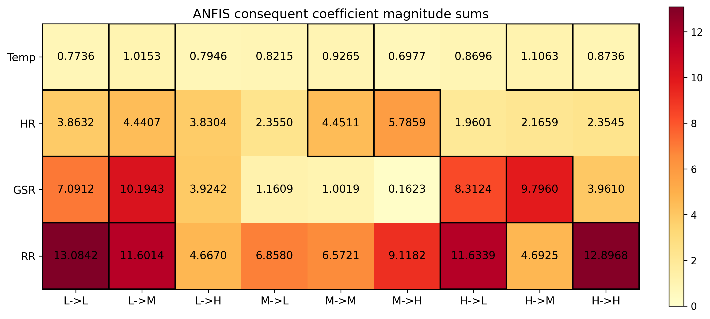
\includegraphics[width=\linewidth]{figures/figure5.png}

\caption{Summed absolute magnitudes of the ANFIS consequent coefficients associated with the fuzzy-transition features.}\label{fig:rId17}

\end{figure}

\subsubsection{Interpretation of Bayesian Evidence}

\begin{figure}[t]

\centering

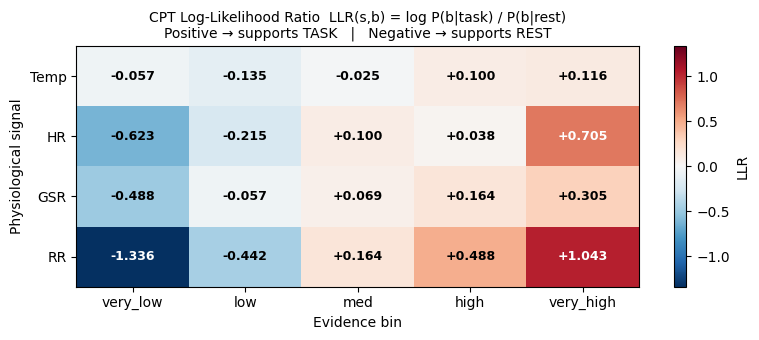
\includegraphics[width=\linewidth]{figures/figure6.png}

\caption{Log-likelihood ratios of the Bayesian evidence bins for the REST and TASK classes.}\label{fig:rId18}

\end{figure}

Figure 6 shows the log-likelihood ratios of the five Bayesian evidence bins. RR provided the strongest class separation, ranging from -1.3366 in the Very Low bin to 1.0433 in the Very High bin, while HR and GSR showed weaker trends and Temp contributed less discriminative evidence. Thus, the BN combined signals according to their class-conditional informativeness. Interpretation stability across retraining remains to be investigated.

\section{Conclusion}

This study proposed an interpretable FTS-ANFIS-BN framework for subject-independent cognitive-load classification using Temp, HR, GSR, and RR signals. The framework integrates fuzzy transition encoding, signal-specific TSK-ANFIS inference, and soft-evidence Naive Bayes fusion. Model configuration and the decision threshold were selected exclusively from participant-level out-of-fold predictions. On the independent hold-out set of 193 samples from five unseen participants, the proposed model achieved 0.7513 accuracy, 0.7519 balanced accuracy, 0.7447 TASK F1-score, and 0.7734 ROC-AUC. The proposed framework outperformed the evaluated machine-learning baselines, while the ablation results supported the contributions of ANFIS inference and Bayesian fusion. Its intermediate representations also enabled interpretation through fuzzy transitions, ANFIS consequent coefficients, and Bayesian evidence. The main limitations are the small participant cohort, evaluation on a single dataset, the Naive Bayes conditional-independence assumption, and the lack of explanation-stability analysis. Future work should evaluate larger datasets, assess interpretation stability, and investigate more flexible yet interpretable Bayesian structures.

\begin{credits}\subsubsection{Competing interests}

The authors declare no conflict of interest.

\subsubsection{Author contributions}

Conceptualization and supervision, Q.H.N. and N.T.D.; methodology, analysis, and original draft preparation, L.T.M.H.; software, data curation, and visualization, L.T.M.H. and Q.D.M.; validation and resources, D.T.N.; review and editing, Q.H.N., N.T.D., D.T.N., L.T.M.H., and Q.D.M. All authors have read and agreed to the published version of the manuscript.

\subsubsection{Acknowledgments}

The authors would like to thank Saigon University, Vietnam, for academic support.

\end{credits}

\begin{thebibliography}{22}

\bibitem{ref1} J. Sweller, "Cognitive load during problem solving: Effects on learning", Cognitive Science, Vol. 12, No. 2, pp. 257-285, 1988.

\bibitem{ref2} M. Gjoreski, T. Kolenik, T. Knez, M. Luštrek, M. Gams, H. Gjoreski, and V. Pejović, ``Datasets for cognitive load inference using wearable sensors and psychological traits'', Applied Sciences, Vol. 10, No. 11, Article 3843, 2020.

\bibitem{ref3} M. Gjoreski, B. Mahesh, T. Kolenik, J. Uwe-Garbas, D. Seuss, H. Gjoreski, M. Luštrek, M. Gams, and V. Pejović, ``Cognitive load monitoring with wearables: Lessons learned from a machine learning challenge'', IEEE Access, Vol. 9, pp. 103325--103336, 2021.

\bibitem{ref4} S. G. Hart and L. E. Staveland, "Development of NASA-TLX (Task Load Index): Results of empirical and theoretical research", Advances in Psychology, Vol. 52, pp. 139-183, 1988.

\bibitem{ref5} Q. Song and B. S. Chissom, "Fuzzy time series and its models", Fuzzy Sets and Systems, Vol. 54, No. 3, pp. 269-277, 1993.

\bibitem{ref6} W. Pedrycz, K. Hirota, and S. Sessa, "A decomposition of fuzzy relations", IEEE Transactions on Systems, Man, and Cybernetics, Part B, Vol. 31, No. 4, pp. 657-663, 2001.

\bibitem{ref7} J. S. R. Jang, "ANFIS: Adaptive-network-based fuzzy inference system", IEEE Transactions on Systems, Man, and Cybernetics, Vol. 23, No. 3, pp. 665-685, 1993.

\bibitem{ref8} J. Pearl, Probabilistic Reasoning in Intelligent Systems: Networks of Plausible Inference, Morgan Kaufmann Publishers, San Francisco, 1988.

\bibitem{ref9} S. Iarlori, D. Perpetuini, M. Tritto, D. Cardone, A. Tiberio, M. Chinthakindi, C. Filippini, L. Cavanini, A. Freddi, F. Ferracuti, A. Merla, and A. Monteriù, ``An overview of approaches and methods for the cognitive workload estimation in human--machine interaction scenarios through wearables sensors'', BioMedInformatics, Vol. 4, No. 2, pp. 1155--1173, 2024. doi:10.3390/biomedinformatics4020064.

\bibitem{ref10} C. Anders, S. Moontaha, S. Real, and B. Arnrich, ``Unobtrusive measurement of cognitive load and physiological signals in uncontrolled environments'', Scientific Data, Vol. 11, Article 1000, 2024. doi:10.1038/s41597-024-03738-7.

\bibitem{ref11} H. Kim, M. Kim, and Y. Han, ``Models for classifying cognitive load using physiological data in healthcare context: A scoping review'', Applied Sciences, Vol. 15, No. 16, Article 9155, 2025. doi:10.3390/app15169155.

\bibitem{ref12} W. K. Wang, I. Chen, L. Hershkovich, J. Yang, A. Shetty, G. Singh, Y. Jiang, A. Kotla, J. Z. Shang, R. Yerrabelli, A. R. Roghanizad, M. M. H. Shandhi, and J. Dunn, "A systematic review of time series classification techniques used in biomedical applications", Sensors, Vol. 22, No. 20, Article 8016, 2022. doi:10.3390/s22208016.

\bibitem{ref13} T. Thamaraimanalan, D. Gopal, S. Vignesh, and K. Kishore Kumar, "Exploiting adaptive neuro fuzzy inference systems for cognitive patterns in multimodal brain signal analysis", Scientific Reports, Vol. 15, Article 9029, 2025. doi:10.1038/s41598-025-93241-9.

\bibitem{ref14} P. Y. Zhou and K. C. C. Chan, "Fuzzy feature extraction for multichannel EEG classification", IEEE Transactions on Cognitive and Developmental Systems, Vol. 10, No. 2, pp. 267 279, 2018. doi:10.1109/TCDS.2016.2632130.

\bibitem{ref15} P. O. Lucas, O. Orang, E. M. A. M. Mendes, P. C. L. Silva, and F. G. Guimaraes, "A tutorial on fuzzy time series forecasting models: Recent advances and challenges", Learning and Nonlinear Models, Vol. 19, No. 2, pp. 29-50, 2021.

\bibitem{ref16} Y. Pan, L. Zhang, Z. Li, and L. Ding, "Improved fuzzy Bayesian network-based risk analysis with interval-valued fuzzy sets and D-S evidence theory", IEEE Transactions on Fuzzy Systems, Vol. 28, No. 9, pp. 2063-2077, 2019.

\bibitem{ref17} J.-K. Kim, K. Lee, and S. G. Hong, ``Cognitive Load Recognition Based on T-Test and SHAP from Wristband Sensors'', Human-centric Computing and Information Sciences, Vol. 13, pp. 1--14, 2023. doi:10.22967/HCIS.2023.13.027.

\bibitem{ref18} T. J. Ross, Fuzzy Logic with Engineering Applications, 3rd ed., John Wiley \& Sons, Chichester, 2010.

\bibitem{ref19} M. Sugeno and G. T. Kang, "Structure identification of fuzzy model", Fuzzy Sets and Systems, Vol. 28, No. 1, pp. 15-33, 1988.

\bibitem{ref20} J. Dougherty, R. Kohavi, and M. Sahami, "Supervised and unsupervised discretization of continuous features", In: Proc. of the Twelfth International Conference on Machine Learning, pp. 194-202, 1995.

\bibitem{ref21} S. F. Chen and J. Goodman, "An empirical study of smoothing techniques for language modeling", In: Proc. of the 34th Annual Meeting of the Association for Computational Linguistics, pp. 310-318, 1996.

\bibitem{ref22} Y. Peng, S. Zhang, and R. Pan, ``Bayesian network reasoning with uncertain evidences'', International Journal of Uncertainty, Fuzziness and Knowledge-Based Systems, Vol. 18, No. 5, pp. 539-564, 2010

\end{thebibliography}

\end{document}